% 第2章
\section{関連研究}
  \label{sec:関連研究}
    \par
  
  \subsection{シェアサイクルの現状と課題}
    \label{sec:シェアサイクルの現状と課題}
      \par シェアサイクルは,都市部を中心に世界各地で普及している持続可能な交通手段であり,そのビジネスモデルは主にBtoC型である.本節では,これらのモデルの現状と課題について検討し,特にBtoC型シェアサイクルの限界とCtoC型シェアリングエコノミーの動向に焦点を当てる.
      \par シェアサイクルの分野でも,CtoC型モデルを導入することによって,BtoC型のシェアサイクルビジネスモデルが抱える課題を解決し得る可能性がある.遊休自演者の有効活用や,需要に応じた柔軟なサービス提供,初期投資や運営コストの削減など,CtoC型ならではのメリットが期待される.
      
      \subsubsection{BtoC型シェアサイクルの限界}
        \label{sec:BtoC型シェアサイクルの限界}
          \par BtoC型(Business-to-Consumer)シェアサイクルとは,事業者が自転車を保有および運営し,利用者がそのサービスを利用して自転車を借りるというビジネスモデルである.BtoC型では,特定の企業や自治体が自転車を大規模に保有・管理し,ユーザが自転車が駐輪されているステーションや無人ポートから自転車を借りる.欧米やアジアなどの大都市を中心として世界的に普及しており,代表的なサービスに,日本のドコモ・バイクシェア,アメリカのCiti Bike,イギリスのSantander Cycles,フランスのVelib’などが挙げられる.
          \par しかし,BtoC型シェアサイクルにはBtoC型であるが故の課題を抱えている.特に初期投資や運営に係るコストの高さや,地理的・時間的再配置の難しさ,自転車ポートの配置や柔軟性・拡張性の制約などが挙げられる.
          \par 世界の40都市における自転車シェアリングシステムの空間的な分布,公共交通機関との統合,および全体的な有効性を分析したMahajan氏らの研究\scalebox{0.7}{\cite{bike-sharing-accessibility}}では,自転車シェアリングサービスのアクセシビリティを評価するための新しい指標であるBSAI(Bike-Share Service Accessibility Index)を導入し,シェアサイクルサービスの利用のしやすさやパフォーマンスを定量的に評価した.
          \par BSAIが高い都市の例として,トロントやワシントン,チューリッヒなどが挙げられている.これらの都市は,広範なサービス範囲や公共交通機関との統合,効率的なインフラ投資を行っているという特徴を持っている.一方で,BSAIが低い都市のの例として,オースティンやサンアントニオなどが挙げられている.これらの都市は,サービス範囲が限定している点や,公共交通機関との連携不足,非効率的なインフラ投資などの課題を持つ点に共通している.
          \par この研究が示唆している課題は,自転車シェアリングシステムのインフラが,都市のすべての住民に公平にアクセス可能ではない点にある.自転車ステーションやポートの分布には地域格差があり,特にBSAIが低い都市ではポートの設置範囲や数が限定されている.それにより,自転車ステーションやポートが特定のエリア内においてのみ利用可能であるため,ユーザのアクセシビリティが悪化している.また,公共交通機関との連携が不足している点も,サービス範囲が限定している点に起因すると考えられる.ただ,BtoC型シェアサイクルでは,企業は利益のために,需要の高い地域に自転車ステーションやポートを設置するはずであるため,必然的な課題とも捉えられる.設置エリア外への展開が難しく,郊外やニッチな需要には対応できない点もBtoC型シェアサイクルの課題である.
          \par また,自転車シェアリング事業の長期的な成功のための政策とビジネス上の教訓を提示することを目的としNikitas氏の研究\scalebox{0.7}{\cite{nikitas2019save}}では,スウェーデンとギリシャでのアンケート調査と,世界各地の自転車シェアリングの成功例と失敗例の分析を組み合わせ,その知見を導き出している.
          \par この研究では,既存の自転車シェアリング事業の成功と失敗の事例を詳細に分析し,その要因を特定している.例えば,アメリカで初めてドックレスバイクシェアシステムを提供した中国のバイクシェアリング企業Bluegogo社は,過剰な自転車供給と需要不足のため,2017年11月に経営破綻した.北京大学発のスタートアップOfo社も,英国事業が赤字となり,2019年1月には3,000台を保有していたロンドンから撤退することとなった.
          \par これらは論文で紹介されいてる事例の一部にすぎないが,この研究が示唆している課題に,過剰共有が挙げられる.ドックレスバイクシェアリングの急速な拡大に伴い,多くの都市で自転車が過剰供給されており,需要と供給のミスマッチが生じていると考えられる.しかし,BtoC型シェアサイクルにおいては,サービスを提供するために大規模な自転車を事前に用意する必要があるため,避けがたい課題である.
          \par 実際に,スウェーデンで実施された,シェアサイクルを利用しない理由を調査した結果を図\ref{fig:自転車シェアリングを頻繁に利用しないまたはまったく利用しない理由}に示す.シェアサイクルサービスを利用しない最大の理由は自身の自転車を所有していることであり,それに続いてシェアサイクルに関わるインフラが不十分であることが,シェアサイクルを利用しない理由の要因として挙げられている.
          \par さらに,地理的・時間的な再配置の難しさについても言及されている.ドックレスバイクシェアリングの導入によって,従来のステーションベースでは不可能であった乗り捨てによるドアツードアの利便性が向上した.その一方で,ユーザによって利用時間帯や場所が偏るため,自転車の分布が不均一になりやすく,需要のある場祖に自転車が不足する,または需要のない場所に自転車が過剰に集中するという課題が発生している.自転車が供給されないまま放置されていると,ユーザのアクセシビリティ低下を招くほか,景観を損ねるなどの,ユーザ以外への影響も懸念される.そのため,定期的に自転車の再配置を行う必要がある.しかし,再配置には人力・トラック等が必要であり,コスト増加やオペレーションの難化を招いている.

          \begin{figure*}[htbp]
            \centering
            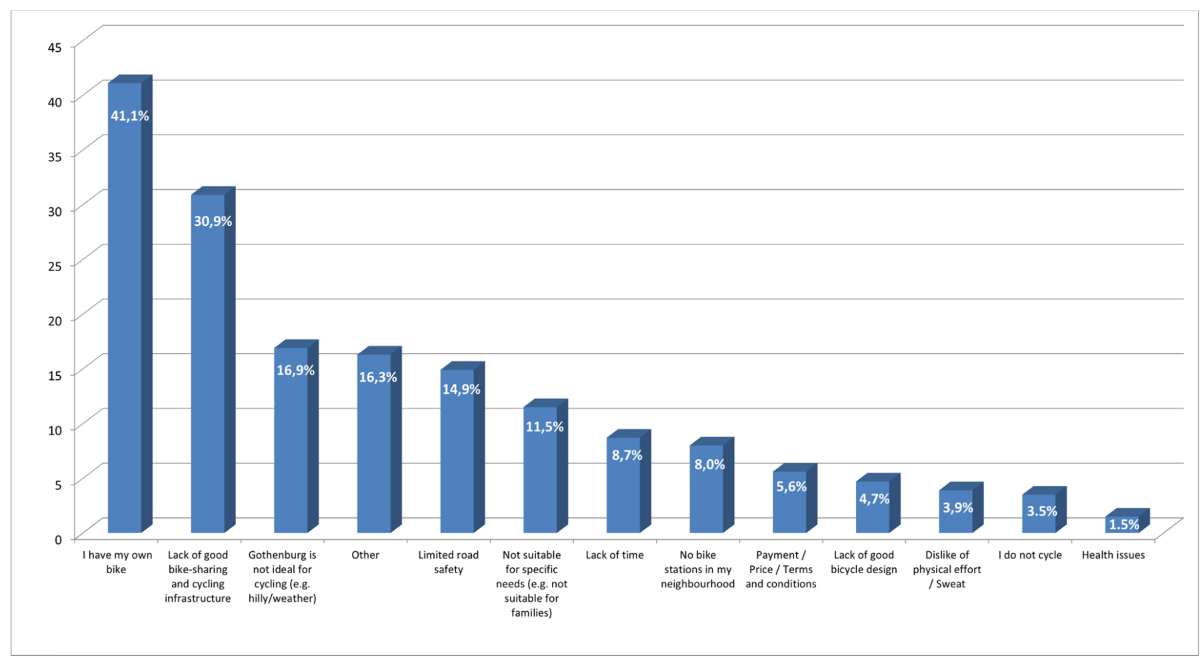
\includegraphics[scale=0.53]
            {figures/reasonsForNotUsingBikeSharing.png}
            \caption{自転車シェアリングを頻繁に利用しないまたはまったく利用しない理由(スウェーデン, ヨーデボリ),How to Save Bike-Sharing: An Evidence-Based Survival Toolkit for Policy-Makers and Mobility Providers\scalebox{0.7}{\cite{nikitas2019save}} より引用}
            \label{fig:自転車シェアリングを頻繁に利用しないまたはまったく利用しない理由}
          \end{figure*}

      \subsubsection{CtoC型シェアリングエコノミーの動向}
        \label{sec:CtoC型シェアリングエコノミーの動向}
          \par シェアサイクルのBtoC型モデルにて例示した課題を受け,様々な事業ドメインにおいてCtoC型シェアリングエコノミーが注目されている.本研究の研究領域であるCtoCシェアサイクルもCtoC型シェアリングエコノミーの一部として捉えることができるため,本項でCtoC型の特徴や動向をまとめ,俯瞰することとする.
          \par まず,CtoC型シェアリングエコノミーを定義するにあたり,Frenken氏らの研究\scalebox{0.7}{\cite{frenken2019putting}} が参考になる.この研究では,シェアリングエコノミーの定義を明確にし,その経済的,社会的,環境的影響を評価し,既存の規制と代替プラットフォームの構造について考察している.Frenken氏らは,シェアリングエコノミーを「消費者が,一時的に,余剰の物理的資産(遊休能力)を,場合によっては金銭を介して相互に利用し合うこと」と定義している.
          \par この定義は,従来の共有の概念とは異なり,特に消費者間の取引であることや遊休能力の活用などが強調されている.つまり,ここで定義しているシェアリングエコノミーは,企業を介さず,消費者同士が直接的に資産を共有し,その共有する資産は,所有者が常に使用しているわけではない余剰の資産(例えば,空いている部屋や使っていない自動車)が共有されることを意味している.ただし,企業はプラットフォーマーとして間接的に取引に介在する可能性はある.これはインターネットプラットフォームの登場により,「見知らぬ者同士の共有(stranger sharing)」という概念が生まれたためである.
          \par シェアリングエコノミーの性質,運営メカニズム,および伝統的な経済理論と市場運営への影響を経済学の観点から詳細に分析することを目的としたChen氏の研究\scalebox{0.7}{\cite{AnalysesAndPerspectivesFromAnEconomicPerspective}}では,具体的な事例分析を通してシェアリングエコノミーの実態を明らかにしている.CtoC型シェアリングエコノミーのプラットフォーム型ビジネスの例として,UberとAirbnbが挙げられる.Uberは,都市交通の分やでドライバーと乗客を結び付け,交通手段の効率化と柔軟な移動オプションを提供し,Airbnbは,住宅所有者が空き部屋を旅行者に貸し出すことを可能にし,宿泊業界に新たな選択肢をもたらした.このような事例から,CtoC型のシェアリングエコノミーおよびそのプラットフォームは,遊休資産を有効活用することで新たな価値を創出し,消費者の行動や産業構造を変化させ,今日の隆盛を迎えるまで成長を遂げてきた.
          \par このCtoC型シェアリングエコノミーの成長と促進の要因は,技術や社会,経済など多岐にわたる.
          \par 協調消費(Collaborative Consumption)への参加を促す動機を調査し,持続可能性や楽しさ,評判や経済的利益といった要因が,協調消費に対する態度や行動意図にどのように影響するかを分析したHamari氏らの研究\scalebox{0.7}{\cite{hamari2016sharing}}では,技術や社会,経済のそれぞれの観点からその要因について言及されている.
          \par 情報通信技術の観点においては,Web2.0の発展により,ユーザ生成コンテンツの増加やオンラインでの共同作業が容易になった点やオンラインプラットフォームを通じて物品やサービスの共有が促進された点,またそれらによってオープンソースソフトウェアやP2Pファイル共有などの様々な形態のシェアリングエコノミーが生まれたことがシェアリングエコノミーの成長要因として挙げられる.
          \par 経済的観点においては,所有することよりもアクセスできることを重視し,必要な時に必要な分だけ利用することに対する消費者の価値観の変化がシェアリングエコノミーの成長を後押ししている.また,CtoCプラットフォームは,従来のサービスよりも安価にサービスを提供できることが多く,消費者にとって魅力的な選択肢となる.例えば,Airbnbはほてるよりも安価な宿泊施設を提供し,Uberはタクシーよりも手頃な価格で移動手段を提供できる場合がある.また,これはユーザだけでなく,提供者としての個人が自分の遊休資産を貸し出すことによって収入を得る機会を提供することにもなる.これによって個人が新たな収入源を確保し,経済的な自立を促進できることも成長要因として挙げられる\scalebox{0.7}{\cite{sundararajan2017sharing}}.
          \par 社会的観点においては,オンラインプラットフォームにおけるユーザレビューや評価システムが,見知らぬ人同士の取引における信頼を構築する上で重要な役割を果たし,個人間でもスムーズに取引が可能となった点が成長要因として挙げられる.また,環境問題意識への関心の高まりから,環境負荷を低減するために持続可能な消費を求める消費者が増加している点も起因していると考えられる.
          \par 本研究とは異なる事業ドメインで構築されているシェアリングエコノミーから着想を得ることで,シェアサイクルの事業ドメインでも応用可能性があると考えられる.
      
  \subsection{スマートロック技術の進展}
    \label{sec:スマートロック技術の進展}
      \par 近年,IoTデバイスの普及に伴い,スマートロック技術は急速に発展してしている.特に,スマートロック技術は,シェアサイクルサービスの実現において重要な役割を果たし,ユーザエクスペリエンスの向上や運用効率の最適化に不可欠な要素となっている.本節では,その技術的進展について,ハードウェアの最新動向およびセキュリティと信頼性の二つの観点から検討する.

      \subsubsection{ハードウェアの最新技術}
        \label{sec:ハードウェアの最新技術}
          \par 前節で言及したBtoCやCtoCモデルへの課題や特徴を踏まえ,本項では,それらを実現・強化するうえで必要となり得るハードウェア技術がどのように発展し,今日を迎えているのかについて理解するため,特にCtoCシェアサイクルサービスに関連するハードウェア基盤の最新動向を概観する.
          \par IoTデバイスのエッジで機械学習(ML)モデルを実行するためのTinyML as a Service(TMLaaS)アーキテクチャを提案したZaidi氏らの研究\scalebox{0.7}{\cite{zaidi2022unlocking}}では,小型で低消費電力MCU(Micro Controller Unit)の発展について触れられている.実際に市販のIoT MCUの消費電力と利用可能なメモリを比較し,理想的にはローカル計算機能を提供するため,RAMやFLASHなどのオンボードメモリが多く,消費電力の低いMCUが必要とされるものの,これらの要件を同時に満たす商用製品は存在しないとまとめられている.しかしそれでも,図\ref{fig:市販のIoT MCUにおける消費電力と使用可能メモリ}に示す通り,最近のESPやSTM,NINA,Nano BLE Senseなどのシリーズは,より高性能でありながら低消費電力を実現しており,設計するにあたってよりよい選択肢となる.
          \par また,組み込みAIやエッジコンピューティングの分野では,AI推論用アクセラレータや小規模ニューラルネット処理が可能なMCUの登場によって,デバイス上での状態判定が実現可能になっている.これはMCUの進化のほか,リソース制約のあるデバイスでMLモデルを開発・実行するためのツールを提供するTinyMLフレームワークや,MCU上でMLを実行するための統一フレームワークであるTensorFlow Lite Micro,ニューラルネットワークモデルの計算量とストレージ要件を削減するための様々なモデル圧縮技術の発展によって実現可能となった.具体的な応用例として,製造業では,振動パターン分析による機械の故障の事前検知やセンサ推論に基づくデバイス制御の自動化,スマート農業では,環境データに基づく農業技術の最適化や,植物の病気の早期検出などが挙げられる.これはシェアサイクル業界においても,振動センサから取得したデータに基づく自転車の状態監視や,加速度センサを用いた自転車の不審な動き検知および盗難の防止にも応用が可能であると推察される.
          \par LPWAN(低電力広域ネットワーク)LoRa/LoRaWANシステムの可能性に焦点を当てているMilarokostas氏らによる研究\scalebox{0.7}{\cite{milarokostas2022comprehensive}}では,LPWAN技術,特にLoRa/LoRaWANシステムに関する包括的な調査を提供しており,通信技術に関する動向を知ることができる.LPWANとは,IoTエコシステムをサポートする主要な候補であり,エネルギー効率が高く,費用対効果の高い技術を組み込んでいるため,IoTサービスプロビジョニングに適している.免許不要のスペクトラム上で無線アクセスを提供する有力なソリューションであるLoRa/LoRaWANや,3GPP(3rd Generation Partnership Project)によって策定されたセルラーIoT(CIoT)技術であり,ライセンススペクトラムを使用するNB-IoTなどがLPWAN技術の例として挙げられる.
          \par これらのLPWAN技術によって,エンドデバイスへのコマンド送信を可能とし,遠隔からのロック制御などの操作も可能となる.さらに,LoRaWANシステムにおいては,ネットワークサーバが位置情報サーバなどの追加コンポーネントを提供できると言及されていることから,位置情報サービスもLoRaWANの応用事例の1つであることが示唆される.これらの技術は,シェアサイクル事業において必要となるGPS追跡や遠隔ロック制御を容易にする基盤技術を提供していると言える.
          \par 通信モジュールやセンサーボード,電源ユニットが標準化され,用途に応じて組み合わせるプラットフォーム的アプローチが容易になっている点もハードウェア技術の進歩に寄与していると考えられる.オープンソースハードウェア(OSH)におけるモジュール性の概念を,デザイン,製造,ハードウェア,コミュニティなど,さまざまな側面から分類し,それぞれのモジュール性を定量的に評価したGavras氏らによる研究\scalebox{0.7}{\cite{Gavras_Kostakis_2021}}では,従来の製品設計の文献で議論されてきたモジュール性とは異なるOSH特有の,無形デザインモジュール性や製造モジュール性などのを提示し,これらのモジュール性がOSHの開発において重要な役割を果たしていることを明らかにしている.
          \par また,ArduinoやRaspberry Pi,ESP32などの開発者コミュニティが拡大し,試作から実用までの開発プロセスが短縮されている点や,第三者が作成した多くのOSHプロジェクトを閲覧できるプラットフォームが発達してきた点も,今日のハードウェア技術基盤を構築する要素になっているに違いない.

          \begin{figure}[htbp]
            \centering
            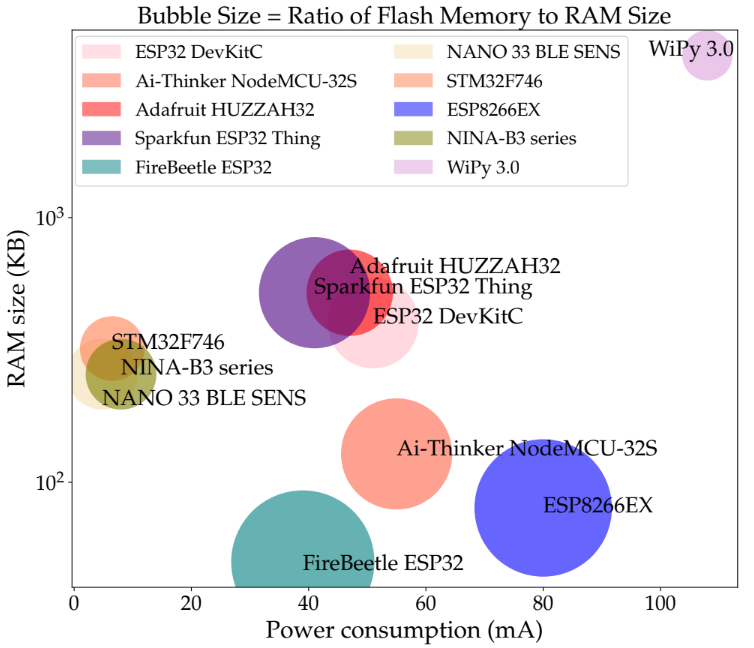
\includegraphics[scale=0.4]
            {figures/powerConsumption.png}
            \caption{市販のIoT MCUにおける消費電力と使用可能メモリ,Unlocking Edge Intelligence through Tiny Machine Learning (TinyML)\scalebox{0.7}{\cite{zaidi2022unlocking}} より引用}
            \label{fig:市販のIoT MCUにおける消費電力と使用可能メモリ}
          \end{figure}
      
      \subsubsection{セキュリティと信頼性の確保}
        \label{sec:セキュリティと信頼性の確保}
          \par スマートロックを含むIoTデバイスにおいてセキュリティリスクや信頼性確保の観点は非常に重要である.特に,本研究の事業ドメインであるシェアサイクルにおいて,機密性や完全性,可用性を以下に守るのか,CtoCサービスでユーザ間の信頼をどう醸成するのかという視点から関連する研究をまとめる.
          \par スマートロックのセキュリティについて調査し,特にMaster LockのBluetoothパッドロックにおける複数の脆弱性を発見したKnight氏らの研究\scalebox{0.7}{\cite{8887393}}では,APIのセキュリティ問題やゲストアクセス権限の不備など,複数の脆弱性を発見および報告し,IoTデバイスのセキュリティにおけるバックエンドサービスの重要性を指摘している.
          \par Master Lockスマートパッドロックに存在した脆弱性は主にAPIセキュリティ上の脆弱性,一時コードにに関する脆弱性,それ以外の脆弱性の3つカテゴリに分類される.APIセキュリティに関しては,本来オーナのみがアクセスできるはずのプライマリーコードをゲストユーザがAPIを通じて取得できてしまう点や,APIが一度生成されると無期限に有効であり,キーが漏洩した場合にユーザのパスワード漏洩と同等のリスクが存在していた点などに脆弱性が報告された.一時コードに関しては,アプリケーションインターフェース上では一時コードの有効期限が4時間と示されていたものの,実際には8時間有効であるという不一致がある点などが報告された.
          \par これらの脆弱性の中でも,特にAPIの脆弱性が最も深刻であり,アクセス権限が無いはずのユーザでもパッドロックを解錠できるという問題があった.CtoCシェアサイクルスキームにおいても,Master Lockのようなスマートロックを使用するため,この脆弱性に対する策を講じる必要がある.具体的には,オーナやゲストといったユーザのステータスに基づき,厳格なアクセス制御ポリシを実装し,不必要な情報へのアクセスを制限したり,APIの呼び出しに対するレート制限を設け,不正なアクセス思考を防止できるようにしたりするアプローチが有効であるとされる.
          \par IoV(Internet of Vehicles)における信頼性管理と信頼性共有のメカニズムを提案したJing氏らの研究\scalebox{0.7}{\cite{jing2022joint}}では,セキュリティと信頼性の確保のために,複数の側面から取り組んでいる.
          \par 信頼性管理メカニズムに関しては,機械学習技術であるRandom Forestを利用して悪意のある車両を識別し,さらに,経路予測アルゴリズムに基づいた信頼性共有メカニズムを導入することで,ネットワーク全体のセキュリティを強化した.また,スライディングタイムウィンドウ技術を用いて過去と現在の記録に基づき,車両の信頼度を総合的に評価し,一時的な行動だけでなく,長期的な信頼性を考慮した評価を可能とした.
          \par 信頼性共有メカニズムに関しては,集中型のコントローラに依存せず,分散型の信頼性管理アプローチを採用し,単一障害の問題を回避することでシステムの拡張性を高めた.また,信頼性情報はRSU(Roadside Units)間でポイントツーポイントで共有され,中央コントローラの負担を軽減し,ネットワークの拡張性を向上させた.
          \par さらに,この研究では通信のセキュリティにも言及されている.Elliptic Curve Cryptography(ECC),Cryptographic Hadh Function,XOR演算を組み合わせた軽量な暗号化メカニズムを導入し,CMV(Cluster-Member-Vehicles),CHV(Cluster-Head-Vehicles),RSU間の通信を保護している.これによって,リソースの限られたIoTおよびIoV環境でも安全な通信を実現することを可能としている.また,暗号化メカニズムによって通信リンクへの攻撃を防ぎ,データの改ざんや盗聴からも保護する役割を担っている.
          \par これらのセキュリティ対策に関する考え方や技術はCtoCシェアサイクルにおけるセキュリティ対策にも応用可能であると考えられる.
          \par スマートシティの様々なアプリケーションとアーキテクチャを紹介し,それらのセキュリティとプライバシーの課題を議論しているZhang氏らの研究\scalebox{0.7}{\cite{zhang2017security}}では,屋外利用のシェアサイクルにも適用可能なセキュリティ設計に関する知見を得ることができる.特に,スマートシティでは,様々なセンサやデバイスを通じてデータが収集され,その中でも位置情報が不可欠な情報として収集される.実際にサービスを提供する際には利用者の同意を得た上で位置情報を取得することが原則であり,その際にデータ収集の目的を明確化し,必要最小限のデータのみを収集するように設計することが求められる.
          
  
  \subsection{マッチングアルゴリズムの研究動向}
    \label{sec:マッチングアルゴリズムの研究動向}
      \par 本節では,シェアサイクルにおける需要と供給を効率的に結びつけるためのマッチングアルゴリズムの研究動向について整理する.マッチングアルゴリズムは,利用者と自転車,自転車と駐輪場,さらにはリソースの最適な割り当てなど,シェアサイクルの運用効率やサービス品質を向上させる上で重要な役割を果たしている.
      \par マッチング問題は,多岐にわたる分野で研究されており,具体的なアプローチとして数理最適化手法と機械学習手法が挙げられる.数理最適化手法では,問題を数奇モデルとして定式化し,制約条件下で目的関数を最適化することで解を求める.一方で機械学習手法では,大量のデータからパターンや特徴を学習し,予測や分類,最適な意思決定を行う.
      \par 本節では,これらの手法がシェアサイクルのマッチング問題にどのように適用されているか,または応用し得るかについて,具体的な研究事例を交えて詳しく述べる.まず,\ref{sec:数理最適化によるマッチング手法}項にて数理最適化によるマッチング手法を取り上げ,その後,\ref{sec:機械学習によるマッチング手法}項にて機械学習によるマッチング手法を概観する.

      \subsubsection{数理最適化によるマッチング手法}
        \label{sec:数理最適化によるマッチング手法}
          \par 本項では,荷物の運搬や配車,リソースの割り当てなどの分野でも盛んに研究されている数理最適化を用いたマッチング手法が,シェアサイクルの需要と供給を効率的に結びつけるためにどのように活用されているか,または活用し得るかを整理する.
          \par まず,マッチング問題の基本定義や典型的な最適化手法やそのモデルについて触れる.整数計画法は,一部または全ての決定変数が整数値のみをとるように制約された線形計画法であり,組み合わせ最適化問題の1つとして広く認知されている\scalebox{0.7}{\cite{wolsey2020integer}}.例えば,荷物の配送計画や工場の生産計画,従業員のシフトスケジューリングなどでは,それぞれ「トラックを何台稼働させるか」「対象製品を何個生産するか」「対象日に従業員を何人割り当てるか」などの問題を解く必要がある.これらは変数が連続値ではなく整数値でなければならない.こうした「整数値でなければならない」という制約を直接扱うための手法が整数計画法である.
          \par 一方で,線形計画法では,決定変数を連続変数として扱うことができるため,ある問題に対して線形計画法によるアプローチで解こうとすると,変数は整数値以外も取ることができる.そのため,本研究でアプローチしているような整数計画問題を線形計画法を用いたプロセスで処理しようとすると,線形計画法による解が整数ではない場合,丸めた解が実行不可能または最適ではない可能性がある\scalebox{0.7}{\cite{hooker2024integer}}.これは,事前に考慮した制約条件の基づき厳密に解を算出した場合でも,丸めてしまうことでとたんに制約条件を満たさない解になる可能性が十分考えられるからである.
          \par このような数理最適化によるマッチング問題を拡張することで,様々な問題にアプローチすることができる.マッチング問題を,選好リストが明示的に与えられる明示的マッチングと,選好リストを予測する暗黙的マッチングの2つに分類し,それぞれの問題に対するモデルとアルゴリズムを包括的にレビューしたRen氏らの研究\scalebox{0.7}{\cite{9416305}}では,特に,検索やユーザとアイテム,エンティティ同士の関係,画像マッチングなどの暗黙的マッチングにおける多様なアルゴリズムを網羅的に扱い,それぞれの応用例と技術的課題について言及されている.
          \par 選好リストが明示的に与えられる明示的マッチングでは,エージェントは合理的かつ利己的であると仮定され,明示的に与えられたランキングとして選好リストを保持している.経済学や数学の分野で主に研究され,結婚市場や医療インターンのマッチングなどが例として挙げられている.安定したマッチングを求める問題に対して用いられることが多い.一方で,選好リストを予測する暗黙的マッチングでは,エージェントの選好は,ユーザーの行動履歴やアイテムの特徴などから推測されるため,データの収集と分析,マッチングスコアを計算するプロセスが重要になる.選好リストを生成するために類似度計算や機械学習が用いられ,ニューラルネットワークなどのアルゴリズムを実装する必要があるマッチング問題で用いられることが多い.より詳細な内容は\ref{sec:機械学習によるマッチング手法}項にて触れるため,適宜参照されたい.
          \par これらの概念は,数理最適化によるマッチング手法をシェアサイクル分野へ応用する際に役立つ可能性がある.明示的マッチングとしては利用者と自転車のマッチングや駐輪場と自転車のマッチングなどのが考えられる.利用者が希望する自転車の条件を考慮した上でマッチング処理を行うことで,より満足度の高いサービスを提供できる.CtoCシェアサイクル領域では特に乗り捨て場所の考慮が重要になるが,これも利用者の目的地と自転車の所有者の位置などを選好リストとして保持することで明示的マッチングが可能となる.
          \par 暗示的マッチングとしては,利用者への自転車の推薦や需要予測と自転車配置の最適化などが挙げられる.利用者の過去の利用履歴や移動パターン,利用時間帯や天気などの様々な情報から,個々の利用者に合った自転車を推薦する際に役立つ.また,シェアサイクルサービス全体としての過去の利用データから需要を予測し,自転車の再配置の最適化などに応用できる可能性も考えられる.
          \par ただ,数理最適化問題を解く際にはNP困難性について考慮しなければならない.NP困難な巡回セールスマン問題を解くため,最短経路や最小全域木などのPクラスのアルゴリズムの知識をニューラルネットワークに組み込むことを試みたGeorgievらの研究\scalebox{0.7}{\cite{np-hard}}では,このNP困難性について触れられている.
          \par 数理最適化におけるNP困難性とは,問題の難しさを示す概念の1つであり,効率的に問題を解くためのアルゴリズムが知られていない問題のことを意味する.問題の規模が大きくなるにつれ,問題を解くための計算量が指数関数的に増加する可能性のある問題である.CtoCシェアサイクルにおける組み合わあせ最適化問題に関しても一般にNP困難問題であることから大規模化するシェアサイクル運用で厳しい計算負荷が生じる可能性がある.そのような場合,従来の数理最適化処理で用いられてきた近似アルゴリズムやヒューリスティックな手法を用い,必ずしも最適ではないかもしれないが,実用的な時間内で十分に良い解を求めるアプローチも選択肢として持っておくべきである.それに加えて,この研究で提案されたニューラルネットワークを用いてNP困難な問題にアプローチする選択肢も存在することを考慮しておけると最適なアプローチを都度選定することができる.
          
      \subsubsection{機械学習によるマッチング手法}
        \label{sec:機械学習によるマッチング手法}
          \par 本項では,\ref{sec:数理最適化によるマッチング手法}項にて扱った数理最適化手法と比較し,機械学習を活用したマッチング手法について概観する.
          \par 数理最適化は,モデルに対して制約や目的関数を定義することで処理を行っているのに対し,機械学習では,大量の履歴データやその特徴量からモデルを学習しマッチングなどの処理を行っている.
          \par このようなデータ駆動型アプローチの特徴については,機械学習の観点から最適化手法を体系的に回顧・要約し,最適化と機械学習の研究の両方の発展に指針を与えることを目指したSun氏らの研究\scalebox{0.7}{\cite{8903465}}にて詳しく解説されている.この研究では,多くの機械学習アルゴリズムの本質は,最適化モデルを構築し,与えられたデータから目的関数のパラメータを学習することであると述べられている.ただ,それ故に,データ量が指数関数的に増加し,モデルの複雑さが増すにつれ,機械学習における最適化手法はますます多くの課題に直面するとも指摘されている.
          \par また,データ駆動型アプローチとしての代表的な機械学習の手法についても紹介されている.半教師あり学習は,教師あり学習と教師なし学習の中間の方法であり,学習プロセス中にラベル付きデータとラベルなしデータの両方を組み込む.ラベル付きデータが少ない状況でもラベルなしデータを活用して学習効果を高めることが可能となる.強化学習では,エージェントが試行錯誤メカニズムを通じて環境と相互作用し,累積報酬を最大化することによって最適な戦略を学習する.環境からのデータを報酬として扱い,その報酬に基づいてエージェントが最適な行動戦略を学習する.メタ学習では,少数のサンプルで新しい環境に効率的に適応できるモデルを設計することを目指している.複数のタスクからのデータに基づいて学習モデルを学習する.その他にも,確率的勾配法やその適応型バリアントが使用された深層学習や,観測データに基づいてモデルのパラメータを最適化し,真の事後分布を近似する変分推論なども紹介されている.
          \par これらの機械学習手法を用い,マッチング手法として具体的にアプローチされている例として,ビジネスインテリジェンスにおける機械学習の応用について焦点を当て,それぞれの特性やツールおよび使用原則を定義したNaneva氏らの研究\scalebox{0.7}{\cite{business-intelligence}}にて紹介されている.
          \par 例えば,ソーシャルメディアにおける顔認識が紹介されている.ソーシャルメディアの最適化を目的として,顔認識機能に機械学習が利用されている.写真の中のポーズや投影をスキャンすることでソフトウェア側が適切な提案を行っている.また,交通渋滞の分析に基づき,交通予測を行うために機械学習が利用されている例も紹介されている.機械学習は項宇宙量の多いエリアと少ないエリアを特定し,ユーザの移動を改善するための定期的な予測を作成することができる.
          \par さらに,Poer BIのようなBIソフトウェアでは,自動機械学習が利用されている.これは,レポートに含まれる情報とは別にデータ操作を提供し,最も関連性の高い特徴とアルゴリズムを自動的に抽出し,機械学習モデルの検証を行う.自動機械学習は,二項予測や一般分類,回帰モデルなどの機械学習モデルを適切に選択して,トレーニング,改善,適用という主要な3つのステップを実行することができる.他にもクラウドサービスのAzureを用いたデータ管理と機械学習の活用についての事例なども紹介されている.
          \par これらの例は,機械学習がビジネスインテリジェンスにおいて,最終的な意思決定をどのように支援するのかを示している.本研究の領域であるCtoCシェアサイクル領域においても利用できる可能性が示唆される.実際に機械学習によるマッチング手法をシェアサイクル領域へ応用されている事例も存在する.ワシントンDCの自転車シェアリングの需要予測モデルを改善するため,交通事故の発生件数という新しい特徴量を機械学習の訓練データとして導入し,その有効性を検証したKim氏らの研究\scalebox{0.7}{\cite{PredictionofBikeShareDemandbyMachineLearning}}を紹介する.
          \par この研究では,ランダムフォレスト,XGBoost,LightGBMという3つの機械学習モデルにこの特徴量を加えることで,RMSLEスコアがどうなるかを検証した.なお,RMSLEとは二乗平均平方根誤差を意味しており,予測値と実際の値の誤差を評価するための指標の1つである.具体的な導出式は以下の\ref{equ:RMSLE}式の通りである.なお,\ref{equ:p_i}式と\ref{equ:a_i}式の通り,$p_i$と$a_i$はそれぞれ予測値と実際の値を意味し,$n$はデータ点の数を意味している.

          \begin{equation}\label{equ:RMSLE}
            \sqrt{\frac{1}{n}\sum_{i=1}^n(\log(p_i + 1) - \log(a_i + 1))^2}
          \end{equation}
          
          \begin{equation}\label{equ:p_i}
            p_i = PredictedValue
          \end{equation}

          \begin{equation}\label{equ:a_i}
            a_i = ActualValue
          \end{equation}

          \par 結果として,すべてのモデルにおいてRMSLEスコアが改善したことが示されている.つまり,シェサイクル領域において,機械学習を用いて需要予測を行う際に多かれ少なかれ交通事故の発生件数が影響していることを示唆している.このようにシェアシェアサイクル領域のみに絞っても機械学習の利用方法は多岐に渡る.
          
  \subsection{API設計と都市への適用性}
    \label{sec:API設計と都市への適用性}
      \par API(Application Programming Interface)は,シェアサイクルシステムにおいてユーザアプリケーションやバックエンドシステム,その他外部サービスやIoT(Internet of Things)を連携させる重要な役割を果たす.APIの技術的な内容については\ref{sec:コア技術の活用}節にて触れる.本節では,APIの設計についての側面や,そのAPIを都市に反映するアプローチ,また,設計および実装を行ったAPIのパフォーマンス評価方法について整理する.
      \par まずはシェアサイクルサービスにおけるAPI設計の要件について概観する.都市におけるデータ統合の観点から,APIをインフラストラクチャの要素として概念化し,都市のデータから新たな接合部を構築する役割を考察したRaetzsch氏らの研究\scalebox{0.7}{\cite{ConceptualizingCityAPIsaselementsofinfrastructures}}では,シェアサイクルサービスのAPI設計を行うにあたって参考になる点が紹介されている.例えば,リアルタイム性の確保についてである.都市のデータ収集や分析を行うにあたってリアルタイムで分析を行うことの重要性や,交通情報や気象条件などのデータをリアルタイムで動的に更新・参照できることの利便性について述べられている.直接言及はされていなかったものの,自転車の利用ステータスや位置情報の取得および更新ができないとクリティカルなインシデントにつながる可能性も危惧される.APIでやり取りするデータはリアルタイム性の確保が必須であると言える.
      \par また,APIを都市に反映するにあたっては,そのスケーラビリティも考慮して設計するべきだとも述べられている.CitySDKプロジェクトを例に挙げ,複数の都市で共通のタスクに対応するためのAPIを開発することで,各都市が個別にサービスを開発する手間を減らし,相互運用性の標準を設定することが重要であるとしている.
      \par さらに,この研究では,都市APIを単なる技術的なツールとしてではなく,都市のインフラストラクチャの一部として捉え,APIの都市への適用についても述べられている.都市インフラストラクチャは,公共サービスを提供するために不可欠であり,エンドユーザにとっては日常生活を送るための当然のものとして認識されている.都市に反映するAPIもそのようなインフラストラクチャとしての公共サービスの一部とする概念である.
      \par 都市へ適応させるにあたってのより具体的なアプローチとして,都市APIは,公共サービスの最適化やビジネスの革新,市民のアクセスと参加の促進などの,異なる利害関係者間で競合する要求を満たすべきであるとしている.また,APIは単なるインターフェースではなく,APIプロデューサとAPIコンシューマとの間でデータ絵のアクセスや利用といった交渉の場であると指摘されている.実際に,都市APIが公共サービスを改善すると同時に,市民や企業が都市データに基づいて新しいサービスを共同で作成できるようにする方法として,前述したCitySDKやOrganicCityのようなプロジェクトが紹介されている.
      \par では,都市に導入したAPIに関するパフォーマンスをどのように評価するのだろうか.ワシントンDCの自転車シェアリングの需要予測モデルを改善するために,交通事故の発生件数という新しい特徴量(外部データソース)を導入し,その有効性を検証したFrança氏らの研究\scalebox{0.7}{\cite{PerformanceEvaluationofRESTandGraphQLAPIsSearchingNestedObjects}}が,APIのパフォーマンス評価のアプローチ方法において参考になる.
      \par APIのパフォーマンス評価は,主に「CPU使用時間」,「メモリ消費量」,「応答時間」,「応答サイズ」の4つの指標に基づいて行われた.CPU使用時間については,CPUが命令を処理するのに要した時間,つまりアプリケーションがCPUを使用した時間の合計をCPUの数で割った値をミリ秒単位で算出して評価した.メモリ消費量については,APIが各検索で使用したメモリの量,つまりアプリケーションが使用したメモリ量を利用可能な総メモリ量で割った割合としてメガバイト単位で算出し評価した.
      \par 応答時間については,各リクエストとその応答の間隔時間,つまりリクエストの開始時刻と応答の受信時刻の差としてミリ秒単位で定義され,評価した.応答サイズについては,各応答のサイズの合計をリクエストの合計数で割ったものとして定義され,REST APIの場合はすべての検索の合計の平均を考量してバイト単位で算出し評価した.
      \par 実際に,この研究では倉庫管理システムを模したシナリオにおいて,ネストされたオブジェクトの検索をRESTとGraphQLのAPIを用いて上記の指標を測定し評価する実験が行われた.なお,これらの指標は,それぞれ独立して測定され,ある指標のログや出力が他の指標の結果に影響を与えないよう配慮されている.また測定ツールとして,Node.jsやPostmanを使用している.
      \par 結果としてはGraphQLがほとんどのシナリオにおいてより優れたパフォーマンスを発揮することが結論付けられている.しかし,本研究においては,APIの評価方法についてのアプローチとしてFrança氏らの研究\scalebox{0.7}{\cite{PerformanceEvaluationofRESTandGraphQLAPIsSearchingNestedObjects}}を参照したまでで,よりハイパフォーマンスであったGraphQLを用いることはない.
